\documentclass[letterpaper]{article}
% Required Packages
\frenchspacing
\usepackage{aaai}
\usepackage{times}
\usepackage{helvet}
\usepackage{courier}
\usepackage{listings}
\lstset{language=Lisp, basicstyle=\footnotesize}
\usepackage{caption}
\DeclareCaptionFont{white}{ \color{white} }
\captionsetup[lstlisting]{singlelinecheck=false, margin=0pt, font={bf,footnotesize}}
\usepackage{graphicx}
\setlength{\pdfpagewidth}{8.5in}
\setlength{\pdfpageheight}{11in}
\nocopyright
% Title
\title{General Game Playing and Monte-Carlo Tree Search}
\author{Armando Ramirez \\ Purdue University, West Lafayette, IN \\ ramirez7@purdue.edu \\ armando.m.ramirez@gmail.com}
% Body
\begin{document}
\maketitle

\section{Introduction}
% TODO (unless no room)
\section{Critique}

\subsection{Background}

\subsubsection{General Game Playing}
The General Game Playing Competition is an annual competition created and managed by Stanford University in which game-playing agents compete by playing games of which they have no prior knowledge.\cite{StanfordGGP} This means they cannot use any heuristical knowledge (unless they can infer some from the game description) and must use more general methods of game-playing instead. Games occur with two or more agents communicating synchronously with a Game Master. The Game Master first tells the agents the rules of the game, and then for the rest of the game it is responsible for receiving player input and telling the players the next state of the game. All moves are synchronous, but turn-based games are simulated by the game rules requiring all but the active player to pass.

All the games played at the competition are described in Game Description Language (also known as Game Definition Language.) Games are boiled down to their most general essence when expressed in this language. A game description is composed of a series of relations. While the game can define its own game-specific relations, there are set relations that must be defined for all games. They are listed below, as described on the Stanford General Game Playing website \cite{StanfordGGP}.
% Remove all this listing crap if I go over-length
\begin{itemize}
\item \emph{role(a)} means that \emph{a} is a role in the game.
\item \emph{base(p)} means that \emph{p} is a base proposition in the game.
\item \emph{input(r,a)} means that \emph{a} is an action for role \emph{r}.
\item \emph{init(p)} means that the proposition \emph{p} is true in the initial state.
\item \emph{true(p)} means that the proposition \emph{p} is true in the current state.
\item \emph{does(r,a)} means that player \emph{r} performs action \emph{a} in the current state.
\item \emph{next(p)} means that the proposition \emph{p} is true in the next state.
\item \emph{legal(r,a)} means it is legal for role \emph{r} to play action \emph{a} in the current state.
\item \emph{goal(r,n)} means that player the current state has utility \emph{n} for player \emph{r}.
\item \emph{terminal} means that the current state is a terminal state.
\end{itemize}

The true and does relations are in effect inputs. The true relations are inputs to the agents from the Game Master, and the does relation is the input from the agents to the Game Master. Therefore, all of the above relations except those two should be defined (most likely partially in terms of true and/or does) in the GDL description of a game.

\subsubsection{Monte-Carlo Tree Search}
Monte-Carlo Tree Search is a combination of the Monte-Carlo method of performing random simulations and game tree search. The algorithm traverses the game tree state by state, and performed random simulations at each state. As it traverses the game tree, the statistics are collected and combined. After the algorithm's budget is exhausted, these statistics are used to make an informed decision.

There are four canonical stages to Monte-Carlo Tree Search \cite{finnsson2012generalized}:
\begin{itemize}
\item \emph{Selection} The algorithm must choose a next-state amongst its explored children. A variety of selection algorithms are used to optimize this choice.
\item \emph{Playout} The Monte-Carlo simulation. A game is played to completion with each player making random moves.
\item \emph{Expansion} The tree begins with just the root node. Each simulation, the tree is expanded, usually by a single node.
\item \emph{Back-Propogation} After a simulation is performed or a terminal state is found, the results must be propogated to all the ancestors of the end state. This is because all its ancestors lead to the result.
\end{itemize}

These stages are visualized in the Figure 1 \cite{finnsson2012generalized}.

\begin{figure}[h]
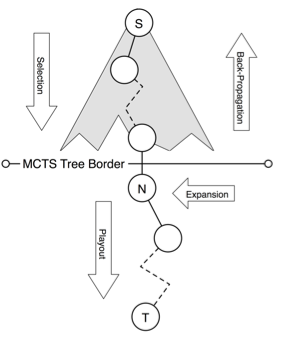
\includegraphics[scale=0.65]{mctsfigure}
\centering
\caption{A single iteration of MCTS visualized}
\end{figure}

\subsection{Generalized Monte-Carlo Tree Search Extensions for General Game Playing}

\subsubsection{Summary}
This paper \cite{finnsson2012generalized} presents extensions menat to be optimization for Monte-Carlo Tree Search that apply to any generally-described game. It is important that this extensions to not make any assumptions about game structure or rules. These extensions aim to improve the execution time and accuracy of the search. Two of them affect the playout stage, which in many games can be quite costly. The final extension affects child selection, which is a key factor in how accurately the agent can traverse the tree.
\begin{itemize}
\item \emph{Goal Stability Early Cutoff} If a trend is confidently found in the progression of the Goal relation of a game, playout can be terminated early and the predicted winner can be stated as the winner.
\item \emph{Terminal Interval Early Cutoff} If a game has a tendency to end in an interval of turns, it is unneccessary to go more than 1/3 of the way through that interval \cite{finnbjorn}
\item \emph{Unexplored Action Urgency} ``Exploit the fringe of the MCTS tree'' by not always exploring all children in the selection phase if the already explored states give enough reason to move on from the current node.
\end{itemize}
% TODO more?

\subsubsection{Critique}

The extensions presented in the paper are all well-thought out and founded within the context of General Game Playing. An extremely conscious effort to avoid domain-specific assumptions is made, and in evaluating the extensions, the author is careful to choose a variety of games with a variety of qualities. The author presents actual results that show that across games, the extensions make nontrivial improvements to Monte-Carlo Tree Search.

However, in practice some of these extensions will end up accomplishing nothing. For example, in many games (such as Tic-Tac-Toe) there is a ternary Goal for every state: a player has either won, lost, or the game is in a state of draw. This goal will not fluctuate from draw until it reaches termination, so Goal Stability Early Cutoff is completely irrelevant to Tic-Tac-Toe.

For more complex games, the Goal Stability Early Cutoff extension is highly dependent on the encoding of the Goal state by the creator of the game description. For instance, in Chess, it would be reasonable to encode the Goal for a player as 100 if they have taken the enemy king, 0 if they have had their king taken, nad 50 if the game is drawn or still in progress. This goal would render the Goal Stability Early Cutoff extension powerless. That said, if the concept of material is introduced into the game, the extension would likely be very useful.

The Unexplored Action Urgency extension represents a key area of research and improvement for MCTS: Selection. In terms of both execution time and accuracy, more powerful Selection algorithms are key.

In the Related Work section, the author notes that some MCTS agents have used similar extensions before; however, \emph{none} have used such extensions without domain-specific knowledge. This paper is relatively recent (2012), and it is reasonable to expect research in General Game Playing Monte-Carlo Tree Search to continue to grow, especially with the recent introduction of GDL-II, which allows for stochastic and imperfect-information games \cite{StanfordGGP}.

\subsection{Understanding the Success of Perfect Information Monte Carlo Sampling in Game Tree Search}

\subsubsection{Summary}
This paper \cite{long2010understanding} is interesting in that it does not aim to explore improvements to MCTS. Instead, it aims to elucidate a previously unresolved problem: MCTS has a great deal of success playing imperfect information games, despite being fundamentally based in perfect information games.

The majority of the paper reasons about the generalized search tree itself, without regard for the actual steps of growing the tree. The paper outlines three basic properties of MCTS search trees for imperfect information games:
\begin{itemize}
\item \emph{Leaf Correlation} The probability that sibling nodes will have the same playoff value. The lower this is, the higher level of control a player has over their chances of winning the game no matter how late in the game it is.
\item \emph{Bias} Whether or not the game favors a player.
\item \emph{Disambiguation Factor} In imperfect information games, the disambiguation factor is how much the possible set of states shrinks as information is revealed.
\end{itemize}

The paper outlines three basic properties of MCTS search trees, and also explains ways to measure these properties at runtime. Once these properties can be measured, the paper goes on to explain how a MCTS agent that is aware of these properties can take advantage of them.

The author performed experiements using both generic synthetic game trees and real games. In both cases, the author's agent was able to take advantage of game tree properties to improve its payoff.

\subsubsection{Critique}

The author does excellent work formalizing properties of Monte-Carlo search trees as they apply to imperfect information games.

The synthetic trees used for testing represent two-player, zero-sum, stochastic imperfect information games. The assumptions of two-player and zero-sum are important and not intrinsic in the domain the paper is discussing, but such games are extremely common so it is natural for the author to use them for his synthetic trees. Despite these trees making these assumptions, they do allow the author to have fine-grained control over the three properties of Leaf Correlation, Bias, and Disambiguation Factor. This leads to a powerful model of MCTS that can be used for repeatable and understandable experiments.

Thankfully, the author did not purely work with synthetic game trees. Real games were used as well to test the ideas presented in the paper. In addition, in real games, the properties must be measured at runtime, whereas in synthetic trees they are known ahead of time. By presenting examples of real games, the author greatly substantiates that his claims operate outside the user-designed synthetic game tree realm.

The author did not discuss General Game Playing; however, with the advent of GDL-II for stochastic and imperfect information games, it is likely that the concepts core to this paper will be used in GDL-II competitions. GDL-II is fairly recent, so it is a vast, unexplored problem space, but in the coming years research such as this author's will be applied to it.

In the conclusion, the author points out that Perfect Information MCTS agents can likely be taken advantage of by actually being predictable in its mistakes. This topic itself merits further discussion, as an agent that actively takes advantage of Perfect Information MCTS would be hugely successful in the General Game Playing arena.

\subsection{MC-RAVE}

\subsubsection{Summary}


\subsubsection{Critique}
This paper is the most specific of the three critiqued. It deals specifically in Go, and less specifically in two-player, perfect information, \emph{zero-sum} games. General Game Playing makes no assumptions about games being zero-sum, so this paper making that assumption greatly limits the domain in which its findings are applicable.

\section{Implementation}

\subsection{Background}

\subsubsection{Clojure}
The implementation of General Game Playing Monte-Carlo Tree Search presented in this paper was implemented in the programming language Clojure. Clojure is a Lisp dialect that can be compiled to run on the Java Virtual Machine, .NET Common Language Runtime, or JavaScript Virtual Machine. It was chosen for a variety of reasons:
\begin{itemize}

\item \emph{Data Structures} Clojure has a rich collection of immutable, persistent data structures including lists, vectors, sets, and maps.
\item \emph{Libraries} Clojure has multiple libraries suited for the project, namely pattern matching and logic programming libraries.
\item \emph{Highly Functional} Clojure has a large set of higher-order functions that can operate over any of its collections.
\item \emph{Homoiconicity} Part of this project involves translating Game Description Language into Clojure. This task was only possible to complete in the allotted timespan because Clojure code is data.
\item \emph{Comfort} On a personal level, I am most comfortable programming in Clojure.
\end{itemize}
\subsubsection{core.logic}

The primary Clojure library used in the implementation was core.logic, which is a port of the logic programming language miniKanren as formulated by William Byrd in his 2010 PhD thesis \cite{byrd2010relational} and by Dan Friedman in his book The Reasoned Schemer \cite{reasonedschemer}.

miniKanren and core.logic are logic programing languages, which means that they deal in relations rather than functions. To get a feel for what that means, consider the + Clojure function compared to the + core.logic relation:

\begin{lstlisting}[frame=single, caption=The + function]
REPL:> (+ 2 3)
5
\end{lstlisting}

\begin{lstlisting}[frame=single, caption=The + relation]
REPL:> (run* [q] (+ 2 3 q))
(5)
REPL:> (run* [q] (+ 2 q 5))
(3)
REPL:> (run* [q] (+ q 3 5))
(2)
REPL:> (run* [q] (+ 2 3 5))
(._0) ;; SUCCESS
REPL:> (run* [q] (+ 2 3 7))
() ;; FAILURE
\end{lstlisting}

(Note: The (\texttt{run* [q] \textless RELATION\textgreater)} macro means ``give me all the values of q such that the relation (with q substituted in accordingly) succeeds'')

There are some key differences:
\begin{itemize}
\item The + function takes two arguments, a and b, and returns a+b, whereas the + relation takes three arguments, a b and c, and is the declaration that a+b=c.
\item This difference allows the relation to run backwards (in effect, performing subtraction.)
\item The relation doesn't return a number. It returns a list of numbers.
\end{itemize}

core.logic also allows the user to declare \texttt{fresh} variables (which are free until bound) to work with. It also provides a relational disjunction in the form of \texttt{conde}. Finally, it offers unification (\texttt{==}) to constrain logic variables. To show these in action (and to show a more complex example of core.logic), consider the below relation and its evaluation:

\begin{lstlisting}[frame=single, caption=Relation to generate all pairs of whole numbers (x y) such that x+y equals 3 or 4]
(defn pair-example [p]
  (fresh [x y]
    (== [x y] p)
    (in x y (interval 0 Infinity))
    (conde
      [(+ x y 3)]
      [(+ x y 4)])))

REPL:> (run* [q] (pair-example q))
([0 3] [0 4] [1 2]
 [1 3] [2 1] [2 2]
 [3 0] [3 1] [4 0])
\end{lstlisting}

This example exposes the under-workings of core.logic: It is, in effect, abstracted search. The user declaratively tells the system what they are looking for, and core.logic performs the search and returns all the solutions it finds. In the context of General Game Playing, these attributes of relations are extremely useful. For example, the legal relation can be used to both generate (via search) all legal moves and check if a move is legal.

\subsection{GDL Translation to core.logic}
\subsubsection{Motivation}
Game Description Language is trivially derived from English. Below are the English and GDL descriptions of legality in Tic-Tac-Toe.
\begin{lstlisting}[frame=single, caption=The Legal relation for Tic-Tac-Toe expressed in English]
;It is Legal for player w to mark cell (m,n)
;if it is true that cell (m,n) is blank and
;it is true that it is player w's turn to
;move. If it is X's turn to move, O can only
;noop. If it is O's turn to move, X can only
;noop. That is, they take turns. 
\end{lstlisting}
\begin{lstlisting}[frame=single, caption=The Legal relation for Tic-Tac-Toe expressed in GDL]
(<= (legal ?w (mark ?m ?n))
    (true (cell ?m ?n b))
    (true (control ?w)))

(<= (legal X noop)
    (true (control O)))

(<= (legal O noop)
    (true (control X)))
\end{lstlisting}

Similarly, a corresponding core.logic relation can be derived from the GDL description.

\begin{lstlisting}[frame=single, caption=The Legal relation translated into core.logic]
(defn legal [role action]
 (conde
  [(fresh [?w ?m?n]
    (== role ?w)
    (== action [:mark ?m ?n])
    (true [:cell ?m ?n :b])
    (true [:control ?w]))]
  [(== role :X)
   (== action :noop)
   (true [:control :O])]
  [(== role :O)
   (== action :noop)
   (true [:control :X])]))
\end{lstlisting}

While the core.logic version is more verbose, each part has a direct correspondence to part of the GDL description:
\begin{itemize}
\item The core.logic relation has an explicit declaration with argument names.
\item All the reflexive relations at the head of each GDL \textless= block are transformed into a series of unifications with the corresponding GDL arguments. 
\item All free variables in the GDL relation are now explicitly declared in a core.logic \texttt{fresh} block.
\item The three separate GDL relations are now combined in a single \texttt{conde} block. In the GDL description, there is an implicit disjunction between the relations, and \texttt{conde} is a core.logic disjunction.
\end{itemize}

Using this core.logic relation, we can accomplish a variety of useful tasks. The below REPL exchange shows the various outputs of the Legal relation for 3x3 Tic-Tac-Toe in the initial state (the entire board is empty and X's turn to move).

\begin{lstlisting}[frame=single,caption=REPL exchange with the core.logic Legal relation for 3x3 Tic-Tac-Toe in the initial state]
;; Legality checking
REPL:> (run* [q] (legal :X [:mark 1 1]))
(._0) ;; SUCCESS
REPL:> (run* [q] (legal :O [:mark 1 1]))
() ;; FAILURE. O cannot mark any square

;; Legal move generation
REPL:> (run* [q] (legal :X q))
([:mark 3 3] [:mark 3 2] [:mark 3 1]
 [:mark 2 3] [:mark 2 2] [:mark 2 1]
 [:mark 1 3] [:mark 1 2] [:mark 1 1])
REPL:> (run* [q] (legal :O q))
(:noop)
\end{lstlisting}
\subsubsection{Implementation}

The implementation presented in this paper can take as input any GDL description (inputted as a list of quoted GDL forms) and create as output runnable core.logic relations. The outputted relations are organized in a Clojure map, where keys are the relation name and values are the runnable relations. This map is hereafter known as the games' \emph{environment}.

The environment is used to accomplish multiple necessary tasks:

\begin{itemize}
\item Relations must be able to reference each other. Because they are read in at runtime, it would be bad practice to use run-time defs.
\item The true and does relation are not static after initialization. During the playing of the game, both of these relations must be constantly updated.
\end{itemize}

 In order to accomplish these tasks, each relation takes an addition argument of the environment. Whenever the relation would make a call to another relation, it instead first fetches the relation from the environment and then calls it. This results in the Legal relation shown above now looking like so:

\begin{lstlisting}[frame=single, caption=The Legal relation translated into core.logic]
(defn legal [env role action]
 (conde
  [(fresh [?w ?m?n]
    (== role ?w)
    (== action [:mark ?m ?n])
    ((env :true) [:cell ?m ?n :b])
    ((env :true) [:control ?w]))]
  [(== role :X)
   (== action :noop)
   ((env :true) [:control :O])]
  [(== role :O)
   (== action :noop)
   ((env :true) [:control :X])]))
\end{lstlisting}

The translation process is fairly straightforward; however, some key steps must be taken due to the relative vagueness of GDL compared to Clojure.
\begin{itemize}
\item \texttt{fresh} variables must be detected in each relation so that they can be explicitly declared. GDL specifies that free variables must start with a question mark, so this task is as simple as walking the syntax and enumerating all symbols that start with \texttt{?}
\item GDL relations are not explicitly grouped. For example, there are multiple relations with Legal as their head, and it is implicit that all these relations are joined by a logical disjunction. The translation algorithm first groups relations by name before transforming their code.
\item Similarly to above, the number of arguments is not declared anywhere. This is also trivial to detect. They are also not named, so gensyms are used to name each variable.
\end{itemize}

After this pre-processing is finished, creating the core.logic relations is as simple as creating code (as Clojure data structures) that represents the relations as a function and then calling \texttt{eval} on that code. The code is created according to the rules exemplified below
\begin{lstlisting}[frame=single, caption=Reflexive head calls turn into unifications]
;; Transforming Legal
(legal ?w (mark ?x ?y))
;; -~->
(== role ?w)
(== move [:mark ?x ?y]
\end{lstlisting}

\begin{lstlisting}[frame=single,caption=All other relations reference the environment]
(true (cell 1 1 b))
;; -~->
((env :true) [:cell 1 1 :b])
\end{lstlisting}

\begin{lstlisting}[frame=single,caption=not turns into negation as failure constraint (nafc)]
(not (line X))
;; -~->
(nafc (env :line) X)
\end{lstlisting}

\begin{lstlisting}[frame=single,caption={\textless= relations are joined in a fresh block}]
(<= (head & args)
    & tail)
;; -~->
(fresh [fresh-vars]
 (transformed head)
 (transformed tail))
\end{lstlisting}

\begin{lstlisting}[frame=single,caption=Multiple related relations are joined by disjunction]
(relation1)
(relation2)
;; ...
(relationN)
;; -~->
(conde
 [(transformed relation1)]
 [(transformed relation2)]
 ;; ...
 [(transformed relationN)])
\end{lstlisting} 

% TODO
% environment
% collect and transform
% eval
% methods for updating true and does relation (membero for true)

\subsubsection{Results}
% TODO: Clean this up and expand
The translation algorithm was tested on four Game Description Language descriptions that can be found on the Stanford Gamemaster website: Tic-Tac-Toe, Chinkook, Chinese Checkers, and Pentago. These games are diverse in factors such as board structure, number of players, types of moves, synchronicity (??) of moves, etc (!!).

\subsection{Monte-Carlo Tree Search}

\subsubsection{Implementation}
My implementation is rather straightforward. It is modularized such that all the explicit steps discussed in a theoretical discussion of Monte-Carlo Tree Search are present and named in the implementation. To aid in programming this algorithm in Clojure, I used a simpler implementation for 3x3 Tic-Tac-Toe as reference \cite{randomcomp}. Because my implementation must work for any game described in GDL, there are some assumptions that can be made about 3x3 Tic-Tac-Toe that cannot be made in a General Game Playing MCTS agent:
\begin{itemize}
\item There can be arbitrary number of players. Therefore, the notion of win, loss, and draw are less relevant. Instead, the raw Goal relation score of each player is used.
\item There are not necessarily turns. If the game is synchronous, the search tree must expand according to all possible combinations of possible moves by all players.

\end{itemize}

The search is itself modularized into an \texttt{iteration} function that can be called a desired amount of times, accumulating statistics with each iteration. This allows for the user to be able to tightly control the amount of resources are used by the search.

\subsubsection{Results}
With a budget as low as 10 iterations, my Monte-Carlo Tree Search algorithm was able to consistently (80\%+ winrate) beat a random player at Tic-Tac-Toe. Its execution time was approximately 2 seconds per turn when running on ECE 207 Redhat computers.

For other games, the execution time was far too long to be reasonable (in large part due to the lengthy playout stages of the games.)

\subsection{Goal Stability Early Cutoff}
\subsubsection{Implementation}
Due to the modular nature of the Monte-Carlo Tree Search code, it was easy to implement the Goal Stability Early Cutoff extension \cite{finnsson2012generalized}. In the playout function, which originally just randomly plays a game to completely, a list of the result of the Goal relation is stored for each player.

Below is a code snippet (with some parts redacted for conciseness) of the core decision making process implemented.
\begin{lstlisting}[frame=single,caption=Clojure implementation of Goal Stability Early Cutoff]
(if (or (terminal? env)
        (and use-early-cutoff?
        (is-goal-stable? goals threshold)
        (>= steps cut)))
     ;; Simulation over
     ;; Return results
     scores
     ;; Simulation not over.
     ;; Choose random child.
     (recur (rand-nth (gen-children env)) 
            next-goals (inc steps)))
\end{lstlisting}

\subsubsection{Results}
The implementation did not break any game that was played using it; however, none of the games that were used for testing had a fine-grained enough Goal relation for the Goal Stability Early Cutoff extension to frequently (or sometimes ever) come into effect.

\section{Future Work}

Of the extensions listed in the critiqued paper, only Finnsson's Goal Stability Early Cutoff extension was incorporated into my Monte-Carlo Tree Search algorithm. Future work would entail implementing a variety of extensions and improvements, including but not limited to UCT, MC-RAVE, Terminal Interval Early Cutoff, and Unexplored Action Urgency. In addition, the game descriptions used from the Stanford Gamemaster website were all for the most part not applicable to the extension implemented, and to some of the extensions not implemented. Future work would examine these extensions in contexts where they are most suited.

The Game Description Language to core.logic transformation algorithm stands to be extremely useful in a variety of contexts. As such, I plan on publishing my work to the appropriate Clojure repositories, such as Leiningen. This would entail a good deal work to make the code publishable, including performing more rigorous testing and writing very thorough documentation.

Finally, the Game Description Language to core.logic transformation algorithm has applications outside of artifical intelligence. It stands to reason that it could be used as the underlying logic of a graphical user interface implementation of a variety of games. Due to the expressivity of Game Description Language, the ability to write the game logic in GDL would vastly speed up the development time of the game engine.

\section{Conclusion}
% TODO (unless no room)

% References
\bibliography{paper}
\bibliographystyle{aaai}
\end{document}
